\documentclass[final]{beamer}
% http://tex.stackexchange.com/questions/56205/wrapfigure-beamer-style
\usepackage{color}
\usepackage{transparent}
%\usepackage{cutwin}
%\usetheme{RJH}
\usetheme{Berkeley}
%\usetheme{Bergen}
\usepackage[orientation=portrait,size=a0,scale=1.4,debug]{beamerposter}
\usepackage[absolute,overlay]{textpos}
\setlength{\TPHorizModule}{1cm}
\setlength{\TPVertModule}{1cm}
\beamertemplatenavigationsymbolsempty
% RGB (145,201,219), #91C9DB
%\definecolor{mybluelabel}{RGB}{145,201,219}
% RGB (48,174,228), #30AEE4
\definecolor{mybluelabel}{RGB}{48,174,228}

\begin{document}
\begin{frame}{} 

%\begin{textblock}{20}(2,2)
%\begin{center}
%\begin{figure}[tbph]
%\centering
%%\includegraphics[width=0.45\textwidth]{dianahep-logo.png}
%
\includegraphics[width=0.70\textwidth]{images/diana-hep-06-logo-horizontal.png}
%\end{figure}
%\url{http://s2i2-hep.org}
%\end{center}
%\end{textblock}



\begin{textblock}{84.0}(1,2)
\begin{center}
%{\transparent{0.2}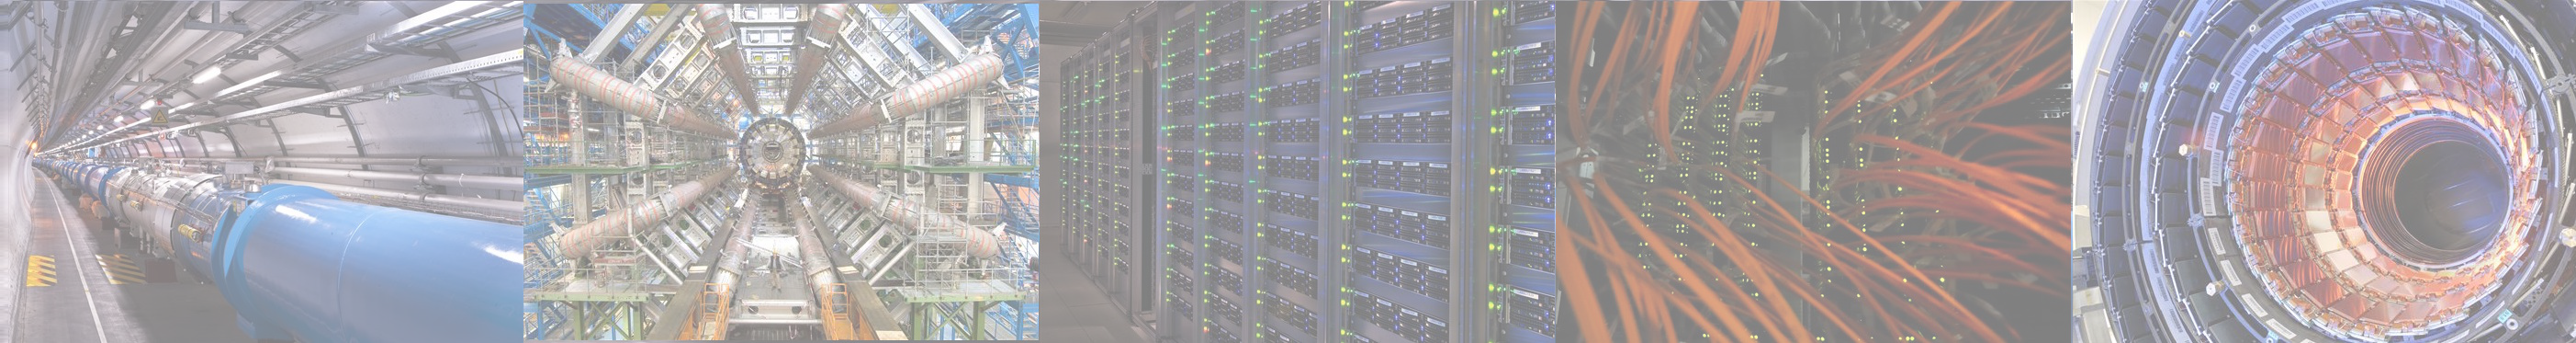
\includegraphics[width=0.95\textwidth]{images/s2i2-banner-50percent.png}}
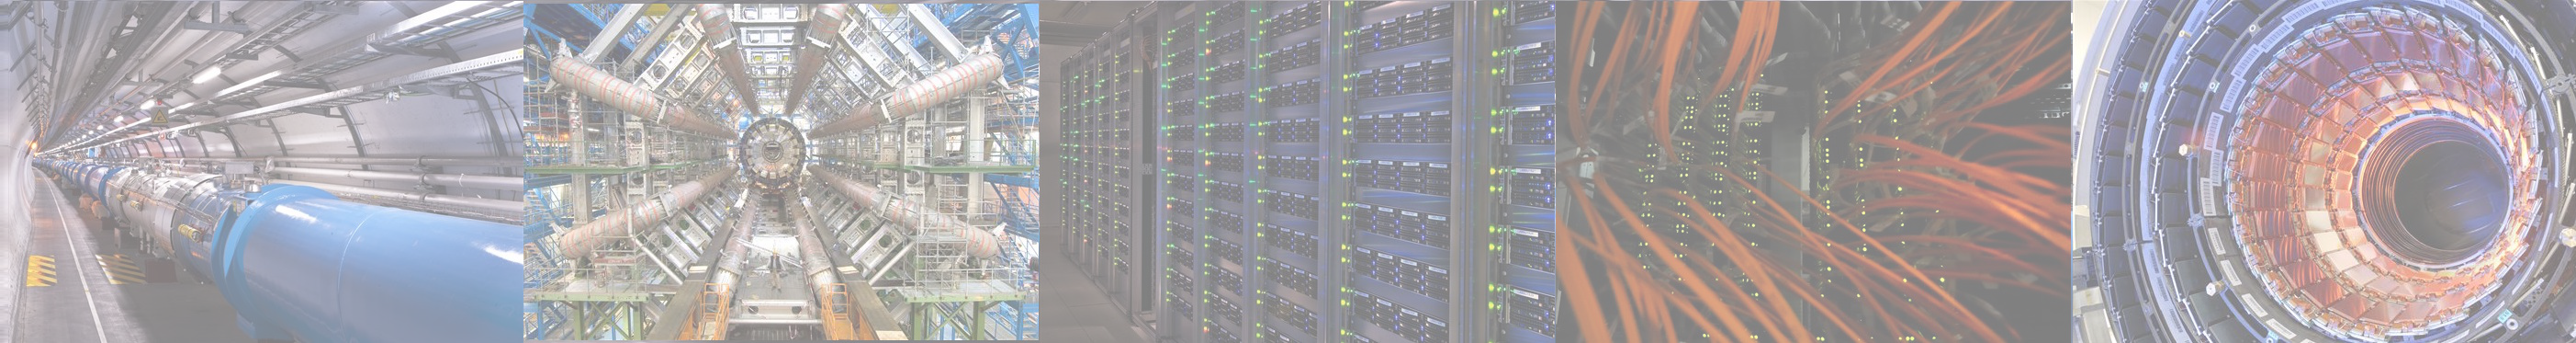
\includegraphics[width=0.95\textwidth]{images/s2i2-banner-50percent.png}
\end{center}
\end{textblock}

\begin{textblock}{84.0}(1,3)
\begin{center}
\begin{Huge}
%\color{white}{
\textbf{
Conceptualization of an S2I2 Institute \\
~~for High Energy Physics (S2I2-HEP)
}
%}
\end{Huge}
\end{center}
\end{textblock}

\begin{textblock}{84.0}(2,8.8)
\begin{center}
\begin{Large}
\textbf{
%PIs: Peter Elmer (Princeton U.), Mark Neubauer (U.Illinois Urbana-Champaign), \\ Mike Sokoloff (U.Cincinnati)
PIs: Peter Elmer (Princeton Univ.), Mark Neubauer (Univ. of Illinois \\ 
at Urbana-Champaign), Mike Sokoloff (Univ. of Cincinnati)
}
\end{Large}
\end{center}
\end{textblock}

\begin{textblock}{78.0}(4,14)
\begin{block}{The S2I2-HEP Project}
The primary goal of the S2I2-HEP conceptualization project is to
prepare a strategic plan for a potential NSF Scientific Software
Innovation Institute (S2I2) to develop software for experiments
taking data in the ``High-Luminosity Large Hadron Collider'' (HL-LHC)
era in the 2020s. In addition, we are working with the HEP Software
Foundation to prepare a larger HEP Community White Paper (CWP)
describing a global roadmap for HEP Software and Computing R\&D for
the 2020s. To this end we are organizing a number of workshops
between Fall 2016 and Summer 2017.
The LHC experiments, for example, use nearly 0.5 Exabyte of
storage today, and planned upgrades through the 2020s will increase this
by more than a factor of 100. 
\end{block}
\end{textblock}

\begin{textblock}{38.0}(4,25)
\begin{block}{High-Luminosity Large Hadron Collider (HL-LHC)}
The primary goal of the S2I2-HEP conceptualization project is to
prepare a strategic plan for a potential NSF Scientific Software
Innovation Institute (S2I2) to develop software for experiments
taking data in the ``High-Luminosity Large Hadron Collider'' (HL-LHC)
era in the 2020s. In addition, we are working with the HEP Software
Foundation to prepare a larger HEP Community White Paper (CWP)
describing a global roadmap for HEP Software and Computing R\&D for
the 2020s. To this end we are organizing a number of workshops
between Fall 2016 and Summer 2017.
The LHC experiments, for example, use nearly 0.5 Exabyte of
storage today, and planned upgrades through the 2020s will increase this
by more than a factor of 100. 
~~~ \\
~~~ \\
\begin{figure}[tbph]
\centering
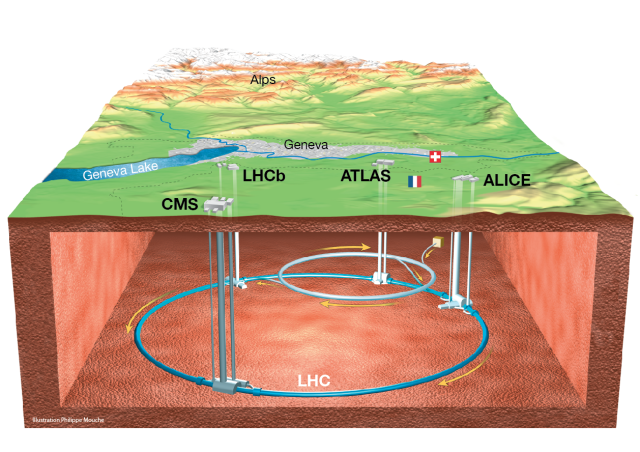
\includegraphics[width=0.96\textwidth]{images/CERN-LHC-cutaway-view-medium.png}
%\begin{center}
%\end{center}
\end{figure}
Reduce size of above image. Timeline picture through 2030s.
\end{block}
\end{textblock}


\begin{textblock}{38.0}(44,25)
\begin{block}{High Energy Physics (HEP)}
%\begin{center}
The quest to understand the fundamental building blocks of nature,
and their interactions, is one of the longest running and most
ambitious of human endeavors. Facilities such as the Large Hadron
Collider (LHC), where we do our research, represent a huge step
forward in our ability to answer these questions. The discovery of
the Higgs boson, the observation of exceedingly rare decays of B
mesons, and exclusion of countless theories beyond the Standard
Model (SM) of particle physics demonstrate that these experiments
deliver results. However, the most interesting fundamental physics
questions remain wide open, amongst them: What is the dark matter
which pervades the universe? Does space-time have additional
symmetries or extend beyond the 3 spatial dimensions we know? What
is the mechanism stabilizing the Higgs mass from enormous quantum
corrections? Are neutrinos, whose only SM interactions are weak,
their own anti-particles? Can the theories of gravity and quantum
mechanics be reconciled? Planned and running HEP experiments 
aim to answer these questions over the next 20 years.
~~~ \\
~~~ \\
\begin{figure}[tbph]
\centering
%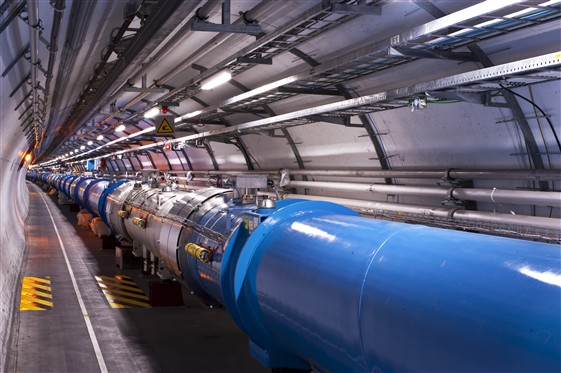
\includegraphics[width=0.48\textwidth]{images/0910152_02-A5-at-72-dpi.jpg}
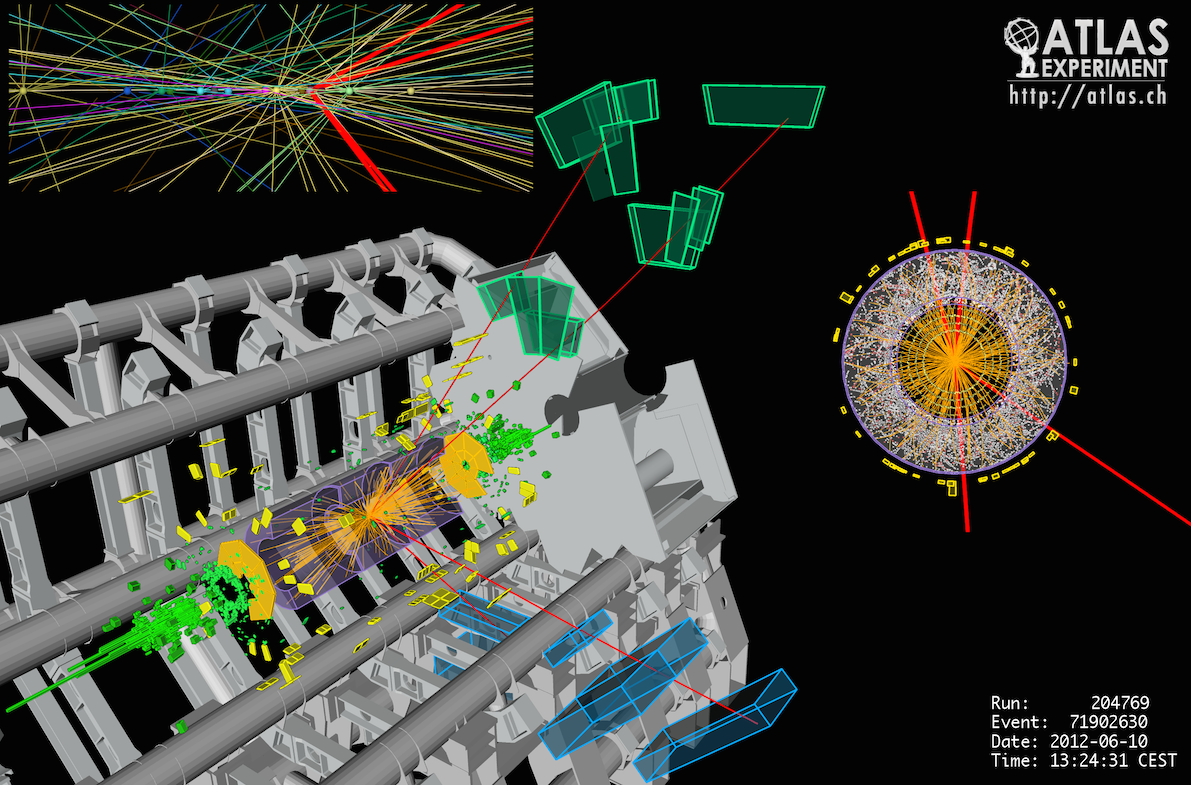
\includegraphics[width=0.41\textwidth]{images/run204769_evt71902630_VP1Base-half.png}
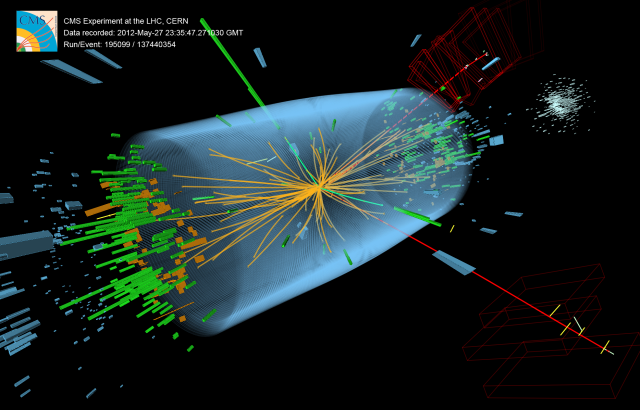
\includegraphics[width=0.42\textwidth]{images/eemm_run195099_evt137440354_ispy_3d-annotated-2.png}
%\begin{center}
%{\small \copyright~2009-2016 CERN (License: CC-BY-SA-4.0)}
%\end{center}
\end{figure}
\end{block}
\end{textblock}

\begin{textblock}{38.0}(44,63)
\begin{block}{The HEP Community and Software Ecosystem}
HEP collaborations, US scientists/students involved in LHC, etc. (Additional text to fill in.)
\end{block}
\end{textblock}


\begin{textblock}{38.0}(44,70)
\begin{block}{The HEP Community and Software Ecosystem}
\begin{figure}[tbph]
\centering
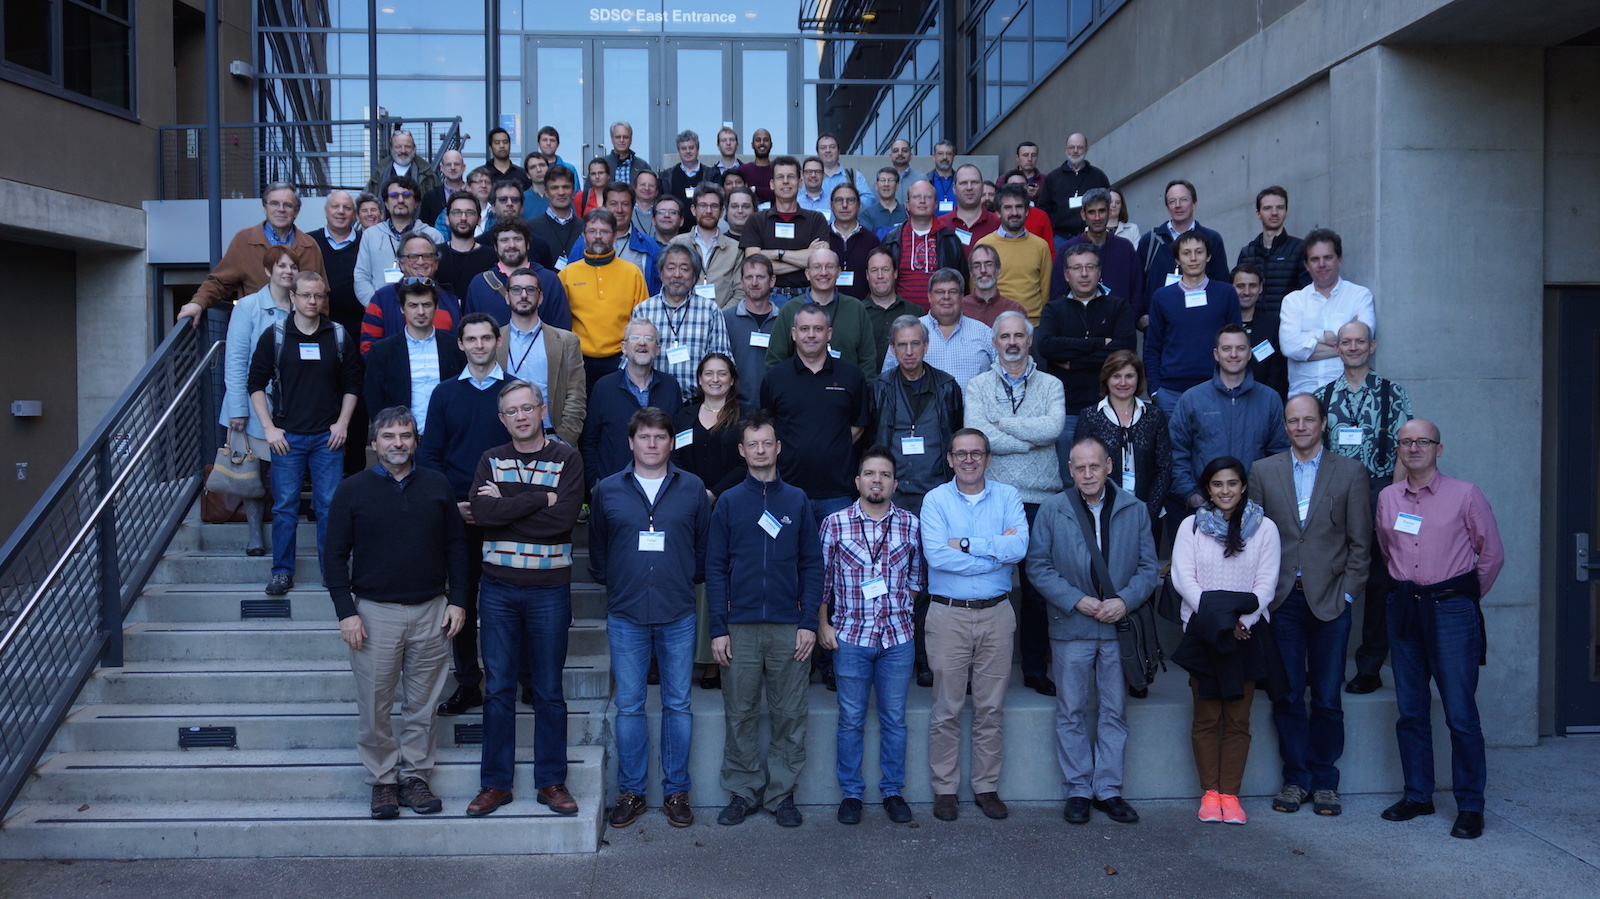
\includegraphics[width=0.80\textwidth]{images/20170125-HSF-SDSC-Workshop-group-photo.jpg}
\end{figure}
\end{block}
\end{textblock}













\begin{textblock}{38.0}(44,107)
\begin{block}{Acknowledgement}
This project is supported by National Science Foundation grants ACI-1558216, ACI-1558219, and ACI-1558233. Any opinions, findings, conclusions or recommendations expressed in this material are those of the developers and do not necessarily reflect the views of the National Science Foundation. \\
%~~\\
%\begin{center}
Images \copyright~2009-2016 CERN (License: CC-BY-SA-4.0)
%\end{center}

\end{block}
\end{textblock}




\end{frame}
\end{document}
